% declare our document type
\documentclass[12pt]{extarticle}

%%%%%%%% PACKAGES NEEDED FOR THIS DOCUMENT

%allow us to create diagrams
\usepackage{tikz}
%used for color
\usepackage{xcolor}
% allow us to put pictures in the document
\usepackage{graphicx}
% this line lets us use larger fonts
\usepackage{extsizes}
% this allows us to create "slides" in the document
\usepackage[many]{tcolorbox}
% this line lets us caption images inside the "slides"
% this is neccesary since the slide doesn't allow the use of
% \figure{} inside
\usepackage{caption}
% sets up tables so that they autoformat
\usepackage{array}
\newcolumntype{L}[1]{>{\raggedright\let\newline\\\arraybackslash\hspace{0pt}}m{#1}}
\newcolumntype{C}[1]{>{\centering\let\newline\\\arraybackslash\hspace{0pt}}m{#1}}
\newcolumntype{R}[1]{>{\raggedleft\let\newline\\\arraybackslash\hspace{0pt}}m{#1}}
% allows use of courier font
\usepackage{courier}
% make the table of contents links like people are used to
% the hidelinks parts hides link outlines
\usepackage[hidelinks]{hyperref}
% resize the margins
\usepackage[margin=1in]{geometry}
% use utf8 encoding
\usepackage[utf8]{inputenc}
% one of the other packages complained until I put this here
\usepackage[english]{babel}
% allow citations
\usepackage{cite}
% code listings
\usepackage{listings}
% fix single quote in listings
\usepackage{textcomp}
\usepackage{filecontents}
%\usepackage[noadjust]{cite}
\usepackage{graphicx}
\usepackage{hyperref}
\usepackage{forest,kantlipsum}
\usepackage{float}
\usepackage{etoolbox}
\usepackage{url}
\usepackage{cleveref}
\usepackage{xcolor}
\usepackage[labelfont=bf]{caption}

%%%%%%%%%%% CUSTOM ENVIRONMENT SETUP

% declare a typesetting environment for code/emphasis
\newcommand{\code}[1]{\texttt{\bfseries#1}}
\newenvironment{codeblock}{\bfseries\texttt\bgroup}{\egroup\par}
% better declaration of font environment
%\DeclareTextFontCommand{\codetext}[1]{\code{#1}}
% declare a large font environment for use in the "slides"
\newcommand{\instruction}[1]{\Large{#1}}
% font environment again
%\DeclareTextFontCommand{\instruction}{\instructionfont}
\newenvironment{instructionblock}{\Large\bgroup}{\egroup}
% declare a "slide" text box for use in the document
% the slide is a numbered \section{}
\newtcolorbox[auto counter]{slide}[3][]{%
colback=brown!5!white,colframe=brown!80!gray,height=3.72in,
title={\addcontentsline{toc}{section}{\thetcbcounter ~~ #2}\bf\Large\thetcbcounter ~ #2\hfill #3 \label{slide \thetcbcounter}\setcounter{section}{\thetcbcounter}}}
% declare a "subslide" text box for use in the document
% the subslide is a numbered \subsection{}
\newtcolorbox[auto counter,number within=section]{subslide}[3][]{%
colback=brown!5!white,colframe=brown!80!gray,height=3.72in,
title={\addcontentsline{toc}{subsection}{\thetcbcounter ~~ #2}\bf\Large\thetcbcounter ~ #2\hfill #3 \label{slide \thetcbcounter}}}
\renewcommand{\labelitemii}{$\circ$}
\lstset{basicstyle=\ttfamily,keywordstyle=\bfseries\color{blue!80!black},identifierstyle=\bfseries,stringstyle=\color{red},showstringspaces=false,commentstyle=\itshape\color{green!40!black},upquote=true}

% My Environments (keep these)
\newcommand{\ben}{\begin{enumerate}}
\newcommand{\een}{\end{enumerate}}
\newcommand{\bi}{\begin{itemize}}
\newcommand{\ei}{\end{itemize}}



%\setlength{\arrayrulewidth}{1mm}
%\setlength{\tabcolsep}{18pt}
%\renewcommand{\arraystretch}{2.5}



%%%%%%%%% SET UP OUR TITLE PAGE

\begin{document}
\title{ Domain Controlling \\ \large Group Policy with Active Directory Part II }
\author{Matt Kirkland \& Jonathan Buch}
\date{March 10, 2017 \\ \hyperref[changelog]{Version 1.5}} %\today
\renewcommand{\abstractname}{Summary}
\begin{titlepage}
\maketitle
\pagenumbering{gobble}
\begin{center}

\includegraphics[scale=.5]{UofI}

\large{CS 439: Applied Security Concepts}

\vskip 40pt

\textbf{Abstract}\\
The purpose of this document is to be a continuation of the material of the Domain Controlling: Group Policy with Active directory document. The tutorial outlined in this document expands on basic knowledge of AD and GPO by having the learner perform AD account management, auditing of group policy, add new group policy, and modify those policies further. The purpose is to acquaint the learner with AD and GPO systems in a very practical sense.

\end{center}


\vfill
\begin{center}
	This work is licensed under a \href{https://creativecommons.org/licenses/by-nc-sa/4.0/legalcode}{Creative Commons Attribution-NonCommercial-ShareAlike 4.0 International License}.
	\vskip 10pt
	
\includegraphics[scale=.5]{cc}
\end{center}

\end{titlepage}

%%%%%%%%%% TABLE OF CONTENTS

\pagebreak
\tableofcontents

%%%%%%%%%%%%%%%%%%%%%%%%%%%%%%%%%%%%%%%%%%%%%%%%%
%%%%%%    BEGINNING OF ACTUAL DOCUMENT
%%%%%%%%%%%%%%%%%%%%%%%%%%%%%%%%%%%%%%%%%%%%%%%%%

\pagebreak
\pagenumbering{arabic}
\setcounter{section}{1}



%-----------------------------------------------------------------------------------------------------------------------------------------------------------------------------------------------------------------%

	\pagebreak
	\begin{slide}{Objectives of this Tutorial}{\hyperref[slide 2]{\textgreater}}
		\begin{instructionblock}
				\ben 
					\item AD account management
					\item Auditing with GPO
					\item Program level policy configuration
				\een
		\end{instructionblock}
	\end{slide}
	\vfill
	
	
%-----------------------------------------------------------------------------------------------------------------------------------------------------------------------------------------------------------------%	
	
	
	\pagebreak	
	\begin{slide}{Required Background}{\hyperref[slide 1]{\textless}\hyperref[slide 3]{\textgreater}}
		%\vskip 10 pt
		\begin{instructionblock}
			\ben
				\item Basic understanding of AD and Group Policy objects
				\item Ability to work with virtual machines (i.e. Virtual Box, VMware, etc.)
				\item Basic understanding of security concepts
			\een
		\end{instructionblock}
	\end{slide}
	
	\pagebreak
	
	
%-----------------------------------------------------------------------------------------------------------------------------------------------------------------------------------------------------------------%

\pagebreak
\begin{slide}{Review of AD and GPO}{\hyperref[slide 2]{\textless}\hyperref[slide 4]{\textgreater}}
	%\vskip 10 pt
	\begin{instructionblock}
	Last time we worked with...
		\ben
			\item Password Policy
			\item Passwords in AD
			\item AppLocker 
		\een
	\end{instructionblock}
\end{slide}

\pagebreak

%-----------------------------------------------------------------------------------------------------------------------------------------------------------------------------------------------------------------%

\pagebreak
\begin{slide}{Questions 1,2}{\hyperref[slide 3]{\textless}\hyperref[slide 5]{\textgreater}}
\begin{instructionblock}
\bi 
\item[Q1:] What utility does AD and GPO provide with regard to password management?
\item[Q2:] Why would you use AppLocker?
\ei

\end{instructionblock}
\end{slide}
\vfill

\vspace{2mm}
\noindent
\textbf{Answer to Q1:}\\
It allows AD admin(s) to set the acceptable length, complexity, and password history along with other options that apply to password creation and use. It can also dictate how passwords are stored and their encryption method.

\vspace{6mm}
\noindent
\textbf{Answer to Q2:}\\
AppLocker has a incredible amount of power over access to files, folders, and applications. It allows a server admin to dictate access to certain parts of a system. As was seen in the last tutorial, AppLocker has the ability to block nearly anything. If used incorrectly, it can cause severe problems for a system. (Principle of Least Privilege)

%-----------------------------------------------------------------------------------------------------------------------------------------------------------------------------------------------------------------%

\pagebreak
\begin{slide}{Challenge: Reactivate Account}{\hyperref[slide 4]{\textless}\hyperref[slide 6]{\textgreater}}
\begin{instructionblock}

Darth's account is locked out. Unlock his account using the Domain Controller (i.e. Windows Server)

\end{instructionblock}
\end{slide} 


%-----------------------------------------------------------------------------------------------------------------------------------------------------------------------------------------------------------------%

\pagebreak
\begin{slide}{Task: Alice's logons}{\hyperref[slide 5]{\textless}\hyperref[slide 7]{\textgreater}}
	\vskip 5pt
	\begin{instructionblock}
		Find Alice's last successful logon attempt \\
		On the Windows 7 VM:
		\ben 
			\item Open up File Manager
			\item Navigate to C: $\rightarrow$ Windows $\rightarrow$ System32 $\rightarrow$ winevt $\rightarrow$ Logs $\rightarrow$ Security
			\item Read the logs and find the last success for Alice
		\een
	\end{instructionblock}
\end{slide}


%-----------------------------------------------------------------------------------------------------------------------------------------------------------------------------------------------------------------%

\pagebreak
\begin{slide}{Task: Auditing Policy Change}{\hyperref[slide 6]{\textless}\hyperref[slide 8]{\textgreater}}
\vskip 5pt
\begin{instructionblock}
	\ben
		\item Open Group Policy Management
		\item Within radicl.security, edit Default Domain Policy
		\item Navigate to $\rightarrow$ Computer Configuration $\rightarrow$ Policies $\rightarrow$ Windows Settings $\rightarrow$ Security Settings $\rightarrow$ Local Policies $\rightarrow$ Audit Policy
		\item Change Audit Policy Change to audit on success
	\een 
\end{instructionblock}
\end{slide}

%-----------------------------------------------------------------------------------------------------------------------------------------------------------------------------------------------------------------%
\pagebreak
\begin{slide}{Challenge: Account Lockout}{\hyperref[slide 7]{\textless}\hyperref[slide 9]{\textgreater}}
	\vskip 5pt
	\begin{instructionblock}
	Discover why Darth's account was locked out.
	\end{instructionblock}
\end{slide}

	
%-----------------------------------------------------------------------------------------------------------------------------------------------------------------------------------------------------------------%

\pagebreak
\begin{slide}{Task: Adding Group Policy (Win Server VM)}{\hyperref[slide 8]{\textless}\hyperref[slide 10]{\textgreater}}
\vskip 5pt
\begin{instructionblock}
	\ben 
		\item Open the policy\_templates folder on the desktop. Navigate to windows $\rightarrow$ admx and copy chrome.admx
		\item Then, navigate to Computer $\rightarrow$ Local Disk C: $\rightarrow$ Windows $\rightarrow$ PolicyDefinitions and paste the chrome.admx here 
		\item Navigate back to policy\_templates $\rightarrow$ windows $\rightarrow$ admx $\rightarrow$ en-US and copy the chrome.adml file
		\item Go back to Computer $\rightarrow$ Local Disk C: $\rightarrow$ Windows $\rightarrow$ PolicyDefinitions $\rightarrow$ en-US and paste the chrome.adml here
	\een
\end{instructionblock}
 \cite{ChromeGPO}
\end{slide}
%-----------------------------------------------------------------------------------------------------------------------------------------------------------------------------------------------------------------%


\pagebreak
\begin{slide}{Questions - 3,4}{\hyperref[slide 9]{\textless}\hyperref[slide 11]{\textgreater}}
\begin{instructionblock}
\bi 
\item[Q3:] Why are audits and logs useful?
\item[Q4:] What is the benefit to adding new group policies?
\ei

\end{instructionblock}
\end{slide}
\vfill

\vspace{2mm}
\noindent
\textbf{Answer to Q3:}\\
Audits and Logs are useful because they allow a way to figure out who caused what if a problem occurs. Also, it helps keep users accountable for their actions while on the server. Checking logs and auditing regularly can also catch problems before they occur.


\vspace{6mm}
\noindent
\textbf{Answer to Q4:}\\
The benefit to adding new group policies is being able to configure applications that you add to the server. It lets you choose how an application will function and how a user will be able to use it.


%-----------------------------------------------------------------------------------------------------------------------------------------------------------------------------------------------------------------%
\pagebreak
\begin{slide}{Challenge: Configure Chrome Policy }{\hyperref[slide 10]{\textless}\hyperref[slide 12]{\textgreater}}
\begin{instructionblock}
\ben
	\item Disable developer mode
	\item Set startup pages
	\item Disable ending processes in Chrome Task Manager
	\item Black list "Google"
	\item Set Google Chrome to default browser
\een
\end{instructionblock}
\end{slide}

%-----------------------------------------------------------------------------------------------------------------------------------------------------------------------------------------------------------------%

\pagebreak
\begin{slide}{Questions - 5}{\hyperref[slide 11]{\textless}\hyperref[slide 13]{\textgreater}}
\begin{instructionblock}
\bi 
\item[Q5:] Why is configuring application-level policy important to understand and implement as a server administrator?
\ei

\end{instructionblock}
\end{slide}
\vfill

\vspace{2mm}
\noindent
\textbf{Answer to Q5:}\\
If an administrator couldn't configure Group Policy at the application level, they would have to either completely allow or disallow an application. This gives the administrator a greater degree of granularity when distributing access and usage rights to users.



%-----------------------------------------------------------------------------------------------------------------------------------------------------------------------------------------------------------------%

\pagebreak
\begin{slide}{Conclusion}{\hyperref[slide 12]{\textless}\hyperref[slide 14]{\textgreater}}
	\begin{instructionblock}
	We have looked at...
		\ben
			\item Managing Active Directory accounts
			\item Auditing policy changes and AD users activity
			\item Configuring application level group policy
		\een
	\end{instructionblock}
\end{slide}

%-----------------------------------------------------------------------------------------------------------------------------------------------------------------------------------------------------------------%

\pagebreak
\begin{slide}{Bonus Challenge: Configure IE}{\hyperref[slide 13]{\textless}\hyperref[slide 15]{\textgreater}}
	\begin{instructionblock}
		\ben
			\item Disable developer mode
			\item Disable searching from address bar \& disable search box
			\item Enforce protected mode
		\een
	\end{instructionblock}
\end{slide}

%-----------------------------------------------------------------------------------------------------------------------------------------------------------------------------------------------------------------%
\pagebreak
\begin{slide}{Appendix}{\hyperref[slide 14]{\textless}}
	\begin{instructionblock}
		\ben
			\item Solutions to challenges
			\item Network Diagram
			\item Setup details
			\item Change log
			\item References
		\een
	\end{instructionblock}
\end{slide}
%-----------------------------------------------------------------------------------------------------------------------------------------------------------------------------------------------------------------%
\pagebreak
\textbf{Solutions to Challenges}\\
\ben
	\item \textbf{Challenge: Reactivate Account}
		\ben
			\item On the Windows Sever follow these steps.
			\item In \textbf{Server Manager} go to \textbf{tools} and select \textbf{Active Directory Users and Computers}.
			\item Navigate to \textbf{radicl.security} $\rightarrow$ \textbf{Users} $\rightarrow$ \textbf{Darth}.
			\item Right click and select \textbf{Properties}. Select the \textbf{Account} tab.
			\item Check the box \textbf{Unlock account}. Click \textbf{Apply}.
		\een
	\item \textbf{Challenge: Account Lockout}
		\ben
			\item On the Windows 7 machine follow these steps.
			\item Log in as the local administrator.
			\item Navigate to \textbf{Local Disk (C:)} $\rightarrow$ \textbf{Windows} $\rightarrow$ \textbf{System32} $\rightarrow$ \textbf{winevt} $\rightarrow$ \textbf{Logs} $\rightarrow$ \textbf{Security}. Double click.
			\item Search for the logs stating that Darth failed to log on 4 times. Thus he was locked out.
		\een
	\item \textbf{Challenge: Configure Chrome Policy}\\
Under default domain policy editor, navigate to \textbf{Computer Configuration} $\rightarrow$ \textbf{Administrative Templates} $\rightarrow$ \textbf{Google} $\rightarrow$ \textbf{Google Chrome}. All of the policies are in this folder!
	\item \textbf{Bonus Challenge: Configure IE}\\
	Under default domain policy editor, navigate to \textbf{Computer Configuration} $\rightarrow$ \textbf{Administrative Templates} $\rightarrow$ \textbf{Windows Components} $\rightarrow$ \textbf{Internet Explorer}. All of the policies are in this folder!
\een

%-----------------------------------------------------------------------------------------------------------------------------------------------------------------------------------------------------------------%
\pagebreak
\noindent
\textbf{Network Diagram}\\\\
In order for the tutorial to succeed, the two machines must be connected properly. The Windows Server 2012 R2 (DC) and Windows 7 (domain member) must be on the same network. Static IPs were set to both VMs. For a tutorial on setting static IPs, we recommend: \href{https://support.microsoft.com/en-us/help/15089/windows-change-tcp-ip-settings}{\textbf{Change TCP/IP settings}}. In the section on IPv4 you want to set a manual IP address. Also for the purpose of the tutorial the client needs to set it's DNS IP to be the server's IP. How that is done is also outlined on the linked document. \cite{StaticIP}
\vspace*{20mm}\\
\begin{center}
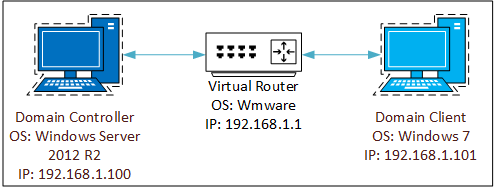
\includegraphics{NetworkDiagram}
\end{center}

%-----------------------------------------------------------------------------------------------------------------------------------------------------------------------------------------------------------------%
\pagebreak
\noindent
\textbf{Setup details}\\\\
In this tutorial, we made use of 2 VMs: Windows Server 2012 R2 (DC) and Windows 7 (domain member). After setting up the network, as outlined in the \textbf{Network Diagram} section, the Server needs to be made a Domain Controller and the client needs to be added to it's domain. The procedure for how to do that is outlined in the previous tutorial: Domain Controlling: Group Policy with Active Directory. See the sections "Setting up Domain" and "Adding Clients".\\
After setting up the Server and Client, a few AD accounts must be made and account policy must be changed. Here we explain how that setup is done.\\\\
\textbf{Set the account lockout threshold, timeout, and authentication failure auditing}\\
On the Windows Server:
\ben
	\item Open Group Policy Management
	\item Within radicl.security, edit Default Domain Policy
	\item Navigate to $\rightarrow$ Computer Configuration $\rightarrow$ Policies $\rightarrow$ Windows Settings $				\rightarrow$ Security Settings $\rightarrow$ Account Policies $\rightarrow$ Account Lockout Policy
	\item Change "Account lockout threshold" to 3 invalid logon attempts. Click "Apply".
	\item Change "Account lockout duration" to 0 minutes.  Click "Apply". This will make it so that any locked account 			must be unlocked by an administrator.
	\item Under Security Settings, navigate to Local Policies $\rightarrow$ Audit Policy.
	\item Change "Audit logon events" to include audits for failures. Click "Apply". This will log failed attempts to 			authenticate a user to the AD server. 
\een
\textbf{Create Darth and Alice's AD Accounts}\\
On the Windows Server:
\ben
	\item Open Active Directory Users and Computers
	\item Within radicl.security, right click on Users and select new $rightarrow$ user.
	\item Fill in the some information and create a password for Darth. Click Finish once done.
	\item Repeat the previous steps to create a user named Alice.
\een
On the Windows Client:
\ben
	\item Invalidly log in to the AD using Darth's account 3 times. You should receive an error message stating that the 		account must be unlocked by an administrator.
	\item Perform only 2 invalid logon attempts for Alice. This should NOT lock her account.
\een


%-----------------------------------------------------------------------------------------------------------------------------------------------------------------------------------------------------------------%
\pagebreak
\textbf{Change Log}\\\\
\label{changelog}

\begin{tabular}{| C{5cm} | C{5cm} | C{5cm} |}
\hline
\textbf{Change(s)} & \textbf{Contributor(s)} & \textbf{Effective Date} \\
\hline
First draft of tutorial & Matthew Kirkland and Jonathan Buch & March 10th, 2017 \\
\hline
Added abstract, network diagram, and expanded Setup details section & Matthew Kirkland & May 10th, 2017 \\
\hline
Correct grammar and spelling errors for final publishing & Jonathan Buch & May 11th, 2017 \\
\hline
Standardized formatting & Ananth Jillepalli & June 15th, 2017 \\
\hline
\end{tabular}

%-----------------------------------------------------------------------------------------------------------------------------------------------------------------------------------------------------------------%
\pagebreak
% this style of bibliography shows urls
\bibliographystyle{IEEEtran}

\begin{thebibliography}{99}

\bibitem{ChromeGPO}

Windows OS Hub, "How to Configure Google Chrome via Group Policies", last accessed 10th March 2017, http://woshub.com/how-to-configure-google-chrome-via-group-policies/, 6th JANUARY 2015.

\bibitem{StaticIP}

Microsoft Support, "Change TCP/IP settings", last accessed 10th May 2017, https://support.microsoft.com/en-us/help/15089/windows-change-tcp-ip-settings, 31st AUGUST 2016.

\end{thebibliography}

\end{document}